%\chapter{涵道风扇式无人机的控制分配问题}
\chapter{自抗扰控制器设计}
%
通过上一章的建模分析,从涵道飞行器的动力学模型可以看出,涵道无人机在飞行过程中受到复杂气动力和气动力矩的影响。对于姿态控制而言,不仅受舵面的驱动力矩作用,还受固定气动面的平衡扭矩、风扇扭矩、陀螺力矩、气动俯仰力矩的作用。这些力矩难以得到其解析形式,但却极大的影响飞机飞行性能。比如,飞机在进行高度控制的过程中需要改变螺旋桨转速,但这同时将因为转速的改变而直接改变系统受到的陀螺力矩、平衡扭矩、风扇扭矩。在存在外扰动时,如果不合理的转换控制力矩到各个舵面偏转角,那么舵面提供的驱动力矩很可能不能抵消这些扰动,从而使系统发散。要使姿态控制更为稳健,首先需要估计这些扰动,对扰动进行补偿之后将控制量转换成舵面偏转角。本节将介绍一种扰动抑制控制算法,将其改进后应用到涵道无人机的姿态控制中。
\section{从PID控制到自抗扰控制}
PID控制器根据系统输入和参考输入的误差进行控制,用误差来消除误差,而不需要知道系统的数学模型。因其参数调节过程简单,参数物理意义明确,在工程实践中得到广泛应用。然而随着科技的发展,工业界对控制器性能的要求越来越高,PID控制的缺点日益明显,主要有:
\begin{enumerate}
	\item PID控制律是基于参考信号与系统输出的误差进行计算的。物理系统的输出通常光滑的,但输入参考信号往往是不光滑的阶跃信号。这一矛盾导致误差的初始值往往比较大,进而使得系统受到较大的冲击产生超调和震荡。为了减小超调,通常是减小控制器增益,但又会使得调节时间变长。即PID控制器存在快速性和超调之间的矛盾。
	\item 实际系统中噪声的存在使得微分器难以实现。
	\item PID控制律是误差的比例、积分、微分的线性组合,组合方式并非最优。
	\item 积分器虽然可以消除静态误差,但会产生积分饱和导致大超调和震荡次数的增加,使系统不稳定。 
\end{enumerate}

针对PID控制的不足,ADRC做了如下改进:
\begin{enumerate}
	\item 为参考输入安排过渡过程:根据系统的阶次安排合适的过渡过程,解决超调和快速性之间的矛盾。使得误差反馈增益的取值范围更大,同时给定的反馈增益能适用于更多的系统,控制器鲁棒性增强。
	\item 提取微分信号:设计非线性微分跟踪器来提取参考输入的微分,降低噪声的影响。同时还设计扩张状态观测器提取反馈信号的微分。
	\item 非线性误差反馈:对误差的比例、微分应用非线性组合构建控制量,得到比线性组合更好的效果。
	\item 估计总和扰动:应用ESO实时估计系统的总和扰动,在控制律中包含扰动补偿,避免了积分反馈的副作用,同时提高了系统抗干扰能力。
\end{enumerate}
\section{自抗扰控制器原理}
自抗扰控制器由跟踪微分器(TD)、扩张状态观测器(ESO)以及非线性误差反馈(NLESF)组成。自抗扰控制技术不依赖于对象的数学模型,通过扩张状态观测器实时估计出包含系统内部模型不确定性和外部扰动不确定性的总扰动,通过动态补偿的方法,将实际系统补偿为积分串联型的标准结构。本节将逐一介绍其原理。
\subsection{跟踪微分器}
物理系统通常有一定的惯性,其状态一般不会突变,而参考输入却可能会是突变信号。因此在跟踪问题中,要求系统跟随突变信号是不合理的。利用跟踪微分器产生参考指令的过渡过程和提取微分信号,使得系统初始误差更为合理。借助微分跟踪器,系统可以使用更大的控制增益,可提高系统快速性。

%设待处理信号为$ v_c(t) $,$ v_c(t) $的微分信号可近似表示为
%\begin{align}
%\dot{v}(t) \approx  \dfrac{1}{T}(v(t)-v(t-T)) 
%\end{align}
%若其变化较平缓,可用小时间常数的惯性环节来近似求取延迟信号,用传递函数表示即
%\begin{align}
%y=\dfrac{s}{T s+1} v_c=\dfrac{1}{T}\left(1-\dfrac{1}{T s+1}\right) v_c  \label{eq_diff}
%\end{align}
%
%越小的时间常数,由式\eqref{eq_diff}近似求得的微分信号越准确。但若待处理信号存在噪声,求得的近似微分信号会将噪声进一步放大。因此考虑下式
%\begin{align}
%\dot{v}_c(t)=\dfrac{v_c\left(t-T_{1}\right)-v_c\left(t-T_{2}\right)}{T_{2}-T_{1}}
%\end{align}
%其中$ T_{1}<T_{2} $。传递函数表达式为
%\begin{align}
%y=\dfrac{1}{T_{2}-T_{1}}\left(\dfrac{1}{T_{1} s+1}-\dfrac{1}{T_{2} s+1}\right) v_c=\dfrac{s}{T_{1} T_{2} s^{2}+\left(T_{1}+T_{2}\right) s+1} v_c
%\end{align}
%若时间常数$ T_{1} $、$ T_{2} $较接近某一数值$ r_0 $,则上式可近似为
%\begin{align}
%y=\dfrac{s}{r^{2}_0 s^{2}+2 r_0 s+1} v_c=s \dfrac{\tau^{2}}{(s+r_0)^{2}} v_c
%\end{align}
%进一步改为一阶微分方程的形式,并在不混淆的情况下省略时间变量$ (t) $,其状态空间实现为
%\begin{align}
%\left\{\begin{array}{l}
%\dot{v}_{1}=v_{2} \\
%\dot{v}_{2}=-r^{2}_0\left(v_{1}-v_c\right)-2 r_0 v_{2} \\
%y=v_{2}
%\end{array}\right.
%\end{align}
%
%形如上式的系统称为线性跟踪微分器,$ v_1 $将跟踪参考输入信号$ v_c(t) $,$ v_2 $将跟踪参考输入的微分信号$ \dot{v}_c(t) $。
%
%为了改进跟踪效果,文献\parencite{HanJingQing_2008}引入了最速综合函数。考虑二阶积分串联型系统
%\begin{align}\left\{\begin{array}{l}
%\dot{v}_{1}=v_{2} \\
%\dot{v}_{2}=u, \quad|u| \leq r_0	\label{eq_second}
%\end{array}\right.\end{align}
%若输入信号取为
%\begin{align}u=-r_0 \operatorname{sign}\left(v_{1}+\dfrac{v_{2}\left|v_{2}\right|}{2 r_0}\right)\end{align}
%则系统\eqref{eq_second}将以最快速度收敛于原点。为了跟踪参考输入$ v_c $,将$ v_1-v_c $代替$v_1$,原系统化为
%\begin{align}\left\{\begin{array}{l}
%\dot{v}_{1}=v_{2} \\
%\dot{v}_{2}=-r_0 \operatorname{sign}\left(v_{1}-v_{c}+\dfrac{v_{2}\left|v_{2}\right|}{2 r_0}\right)
%\end{array}\right.\end{align}
%该系统称为非线性跟踪微分器,它将以最快速度跟踪信号$ v_c $,且$r$越大,收敛速度越快。$ v_2 $可近似认为是踪参考输入的微分信号$ \dot{v}_c(t) $。离散化上述系统可得
%\begin{align}\left\{\begin{array}{l}
%\Psi=-r_{0} \operatorname{sign}\left(v_{1}(k)-v_c(k)+\dfrac{v_{2}(k)\left|v_{2}(k)\right|}{2 r_{0}}\right) \\
%v_{1}(k+1)=v_{1}(k)+h v_{2}(k) \\
%v_{2}(k+1)=v_{2}(k)+h \Psi
%\end{array}\right.\end{align}
%其中$h$为系统采样周期。但此时的系统会产生高频颤振问题,为解决这个问题,考虑将$ \Psi $替换为离散系统的最速控制综合函数$ fst $
%\begin{align}
%{\left\{\begin{aligned}
%	& fst(v_1, v_2, r, h) =-
%	\begin{cases}
%	ra / d &  |a| \leq d,\\
%	r \operatorname{sgn}(a) &  |a| > d.
%	\end{cases}  \\
%	& a  \triangleq
%	\begin{cases}
%	v_{\mathrm{r} 2}+\dfrac{a_{0}-d}{2} sign(n) &  |n|>d_{0},\\
%	v_{\mathrm{r} 2}+n / h &  |n| \leq d_{0}.
%	\end{cases} \\
%	& d  \triangleq r h, d_{0} \triangleq d h, n \triangleq v_1+h v_2 \\
%	& a_{0} \triangleq\left(d^{2}+8 r|n|\right)^{1 / 2}
%	\end{aligned}\right.}
%\end{align}
%其中滤波器因子$r$可取适当大于采样周期$ h $的值$ r=5\sim 10h $,此时跟踪微分器表示为
%\begin{align}\left\{\begin{array}{l}
%fst={fst}\left(v_{1}(k)-v_c(k), v_{2}(k), r, h\right) \\
%v_{1}(k+1)=v_{1}(k)+h v_{2}(k) \\
%v_{2}(k+1)=v_{2}(k)+h fst
%\end{array}\right.	\label{eq_fst}
%\end{align}

有限时间跟踪微分器可设计为如下形式\cite{Guo_2011b}
\begin{align}\left\{\begin{aligned}
\dot{v}_{1}(t) &=v_{2}(t) \\
\dot{v}_{2}(t) &=v_{3}(t) \\
& \vdots \\
\dot{v}_{n}(t) &=R^{n} \Psi \left(v_{1}(t)-v_c(t), \dfrac{v_{2}(t)}{R}, \ldots \dfrac{v_{n}(t)}{R^{n-1}}\right)	
\end{aligned}\right.	\label{eq_h_TD}
\end{align}
当$ R=1$,$v_c=0 $时称为微分器的原系统,并指出当输入$v_c$和函数$\Psi$满足一定条件时该微分跟踪器收敛,我们将在下文给出相应的收敛性结论。基于文献\parencite{Guo_2011b}的结论,我们可以构造如下形式的一类二阶有限时间跟踪微分器
\begin{align}
\left\{\begin{array}{l}
\dot{v}_{1}(t)=v_{2}(t) \\
\dot{v}_{2}(t)=R^{2}\left(-k_{1}\left[v_{1}(t)-v_c(t)\right]^{\alpha}-k_{2}\left[\dfrac{v_{2}(t)}{R}\right]^{\beta}\right)
\end{array}\right.	\label{eq_sec_TD}
\end{align}
其中$ [r]^{\alpha}=\operatorname{sign}(r)\left|r\right|^{\alpha} $,且
\begin{align}
k_{1}, k_{2}>0, \alpha=\dfrac{b-1}{a}, \beta=\dfrac{b-1}{b}, a=b+1, b>1	\label{eq_para_sec_TD}
\end{align}
\subsection{扩张状态观测器}
自抗扰控制的核心是设计扩张状态观测器,对系统未建模动态和外部扰动进行估计。通过在系统中实时补偿该“总和扰动”,使对象模型变成“积分器串联型”线性系统。为简单起见,考虑一个存在外部扰动和内部不确定的二阶系统
\begin{align}
\left\{\begin{array}{l}
\dot{x}_{1}=x_{2} \\
\dot{x}_{2}=f\left(x_{1}, x_{2}, t\right)+w(t)+b u \\
y=x_{1}
\end{array}\right.	\label{eq_sec_sys}
\end{align}
其中$ w(t) $为系统的外部扰动,简记为$ w $,$ f\left(x_{1}, x_{2}, t\right) $为系统内部不确定函数,简记为$ f $。ESO通过将$ f+w $扩充为新的状态$ x_3=f+w $,将上述系统化为
\begin{align}\left\{\begin{array}{l}
\dot{x}_{1}=x_{2} \\
\dot{x}_{2}=x_{3}+b u \\
\dot{x}_{3}=\eta\left(x_{1}, x_{2}, w(t), t\right) \\
y=x_{1}
\end{array}\right.\end{align}
其中$ \eta\left(x_{1}, x_{2}, w(t), t\right) $是未知函数,在ESO设计中,直接忽略该部分。假设参数$ b $已知,设计如下观测器
\begin{align}\left\{\begin{array}{l}
e=\hat{x}_{1}-y \\
\dot{\hat{x}}_{1}=\hat{x}_{2}-\alpha_{1} g_{1}(e) \\
\dot{\hat{x}}_{2}=\hat{x}_{3}-\alpha_{2} g_{2}(e)+b u \\
\dot{\hat{x}}_{3}=-\alpha_{3} g_{3}(e)
\end{array}\right.\end{align}
其中$ \alpha_{i} $为适当的参数,$ g_{i} $为满足一定条件的非线性函数。若满足一定的收敛性条件,上式的$ {z}_{1} $、$ {z}_{2} $将分别收敛于系统状态$ {x}_{1} $、$ {x}_{2} $,$ {z}_{3} $收敛于总和扰动$ f+w $。

若参数$ b $未知,可使用一个估计值$ \hat{b} $代替,该值的估计误差对系统产生的影响作为建模误差一并由$ {z}_{3} $估计,此时$ {z}_{3} $将收敛于新的总和扰动$ f+w+(b-\hat{b})u $。
%将观测器离散化,可表示为
%\begin{align}\left\{\begin{array}{l}
%e=z_{1}-y \\
%{z}_{1}(k+1)={z}_{1}(k)+h(z_{2}(k)-\alpha_{1} g_{1}(e)) \\
%{z}_{2}(k+1)={z}_{2}(k)+h(z_{3}(k)-\alpha_{2} g_{2}(e)+\hat{b} u) \\
%{z}_{3}(k+1)={z}_{3}(k)-h(\alpha_{3} g_{3}(e))
%\end{array}\right.\end{align}

文献\parencite{Guo_2011}给出一种ESO的形式
\begin{align}\left\{\begin{array}{l}
\dot{\hat{x}}_{1}(t)=\hat{x}_{2}(t)+\alpha_{1} \varepsilon\left[\dfrac{y(t)-\hat{x}_{1}(t)}{\varepsilon^{2}}\right]^{a} \\[5mm]
\dot{\hat{x}}_{2}(t)=\hat{x}_{3}(t)+\alpha_{2} \left[\dfrac{y(t)-\hat{x}_{1}(t)}{\varepsilon^{2}}\right]^{2 a-1}+\hat{b}u(t) \\[5mm]
\dot{\hat{x}}_{3}(t)=\dfrac{\alpha_{3}}{\varepsilon}\left[\dfrac{y(t)-\hat{x}_{1}(t)}{\varepsilon^{2}}\right]^{3 a-2}
\end{array}\right.		\label{eq_sec_ESO}
\end{align}
\subsection{非线性误差反馈}
在ADRC控制技术中,延拓了“基于误差来消除误差”的思想。将跟踪微分器得到的跟踪信号以及微分信号与ESO中得到的系统状态的估计信号做差,通过特定的组合产生误差反馈。与PID不同的地方在于,最终的控制量是在误差反馈的基础上添加一个扰动补偿项,将非线性系统线性化。误差反馈使线性化后的系统跟踪给定输入。

由上文可知参考输入$ v_c $经过跟踪微分器得到的过渡过程及其微分信号为$ v_1 $、$ v_2 $,ESO估计的系统状态为$ \hat{x}_1 $和$ \hat{x}_2 $,由此定义状态误差
\begin{align}\begin{array}{l}
e_{1}=v_{1}-\hat{x}_{1} \\
e_{2}=v_{2}-\hat{x}_{2}
\end{array}\end{align}
误差反馈定义为$ u_{0}=\Phi (e_1,e_2) $,常见的误差反馈有
\begin{align}
u_{0} &=k_1 e_{1}+k_2 e_{2} \label{eq_LEF}	\\	
u_{0} &=k_{1} fal\left(e_{1}, \alpha_{1}, \delta\right)+k_{2} fal\left(e_{2}, \alpha_{2}, \delta\right)	\label{eq_NLEF}
\end{align}
其中$ 0<\alpha_{1}<1<\alpha_{2} $,且
\begin{align}
fal(e, \sigma, \xi)=
\begin{cases}
|e|^{\sigma} \operatorname{sgn}(e) &  |e|>\xi,\\
e / \xi^{1-\sigma} &  |e| \leq \xi.
\end{cases}\quad \xi >0
\end{align}
%$ u_0 $还可以有以下几种形式
%\begin{align}\begin{array}{l}
%u_{0}=k_1 e_{1}+k_2 e_{2} \\
%u_{0}=k_1 f a l\left(e_{1}, \alpha_{1}, \delta\right)+k_2 f a l\left(e_{2}, \alpha_{2}, \delta\right), 0<\alpha_{1}<1<\alpha_{2} \\
%u_{0}=-\operatorname{fhan}\left(e_{1}, c e_{2}, r_{0}, h_{0}\right)
%\end{array}\end{align}
%式\eqref{eq_LEF}称为线性误差反馈,式\eqref{eq_NLEF}称为非线性误差反馈。
结合扩张状态观测器估计到的总和扰动$ z_{3} $,则总的控制律为
\begin{align}
u=\dfrac{u_{0}-z_{3}}{\hat{b}}=\dfrac{1}{\hat{b}}(\Phi (e_1,e_2) -z_{3})
\end{align}
此时式\eqref{eq_sec_sys}所示被控对象对应的闭环系统变为积分串联型系统
\begin{align}\left\{\begin{array}{l}
\dot{x}_{1}=x_{2} \\
\dot{x}_{2}=\Phi(e_1,e_2) \\
y=x_{1}
\end{array}\right.\end{align}
整个闭环系统结构框图如图\ref{fig_ADRC}所示
\begin{figure}[htbp]
	\centering	
	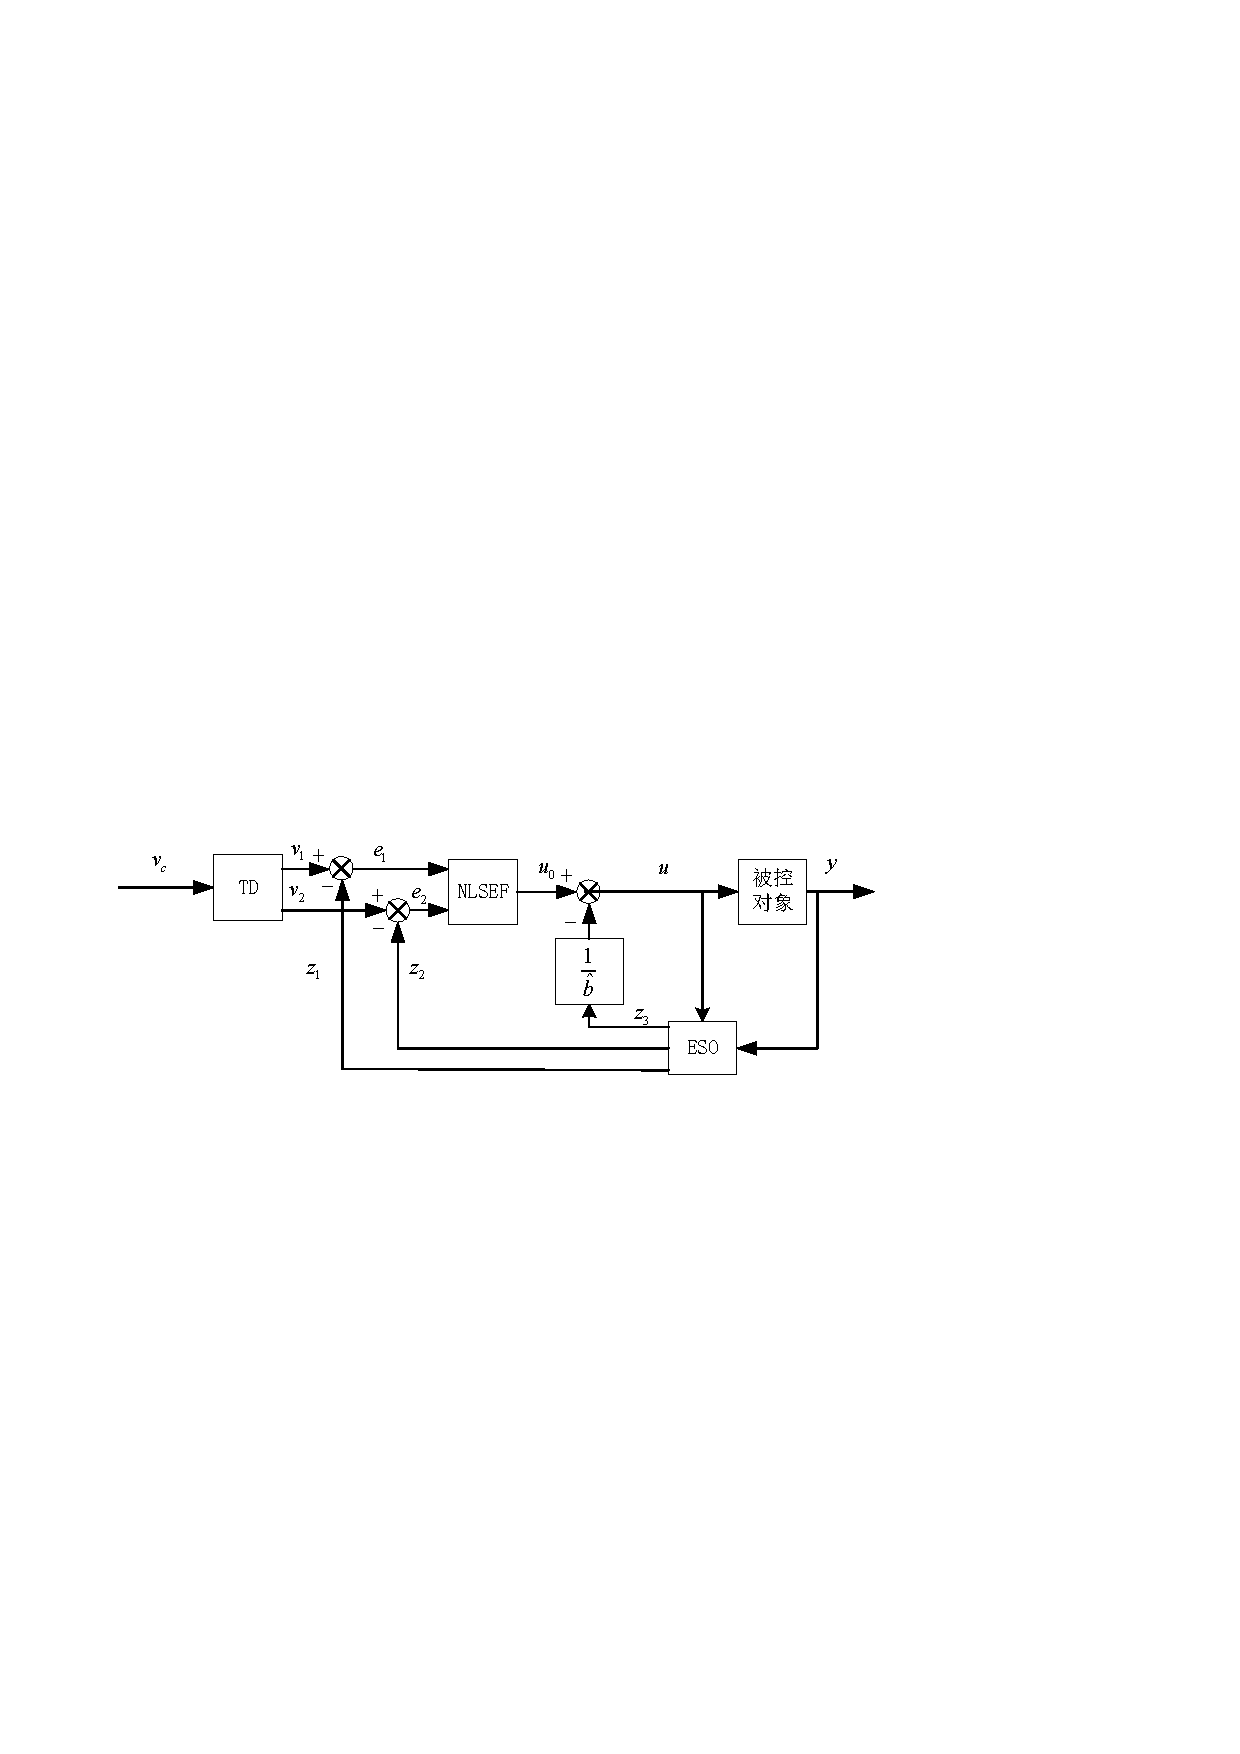
\includegraphics[scale=1]{Fig/Fig_ADRC.pdf}
	\caption{\label{fig_ADRC}自抗扰控制器结构框图}
\end{figure}
\section{自抗扰控制的收敛性条件}
ADRC的收敛性分析可以分为三部分:一是TD的收敛性;二是ESO的收敛性;三是使用NLESF的闭环系统的收敛性。ADRC的收敛性最初由文献\parencite{HanJingQing_2008}给出分析。近年来,郭宝珠等人给出了更严格的数学证明,在文献\parencite{Guo_2010,Guo_2011b,Guo_2011c,Guo_2011d}给出了跟踪微分器的收敛性证明。文献\parencite{Guo_2011,Guo_2011a,Guo_2012,Zhao_2016e}给出了扩张状态观测器的收敛性证明,文献\parencite{Guo_2013,Zhao_2016a,Guo_2013,Guo_2012a}分析了ADRC闭环系统的收敛性。本文为了后续方便选择ADRC中的参数以及相关的非线性函数,不加证明地给出几条定理。
\subsection{跟踪微分器的收敛性}
对式\eqref{eq_h_TD}所示的跟踪微分器,文献\parencite{Wang_2007}给出了这类跟踪微分器在强条件下的收敛性证明,即要求有一个李雅普诺夫函数使TD的原系统全局渐进稳定且该李雅普诺夫函数是全局Lipschitz连续的。而文献\parencite{Guo_2011b}指出收敛性证明不再需要全局Lipschitz连续的李雅普诺夫函数,弱化了收敛性证明所需的条件,得到如下定理:
\begin{theorem}
	若跟踪微分器\eqref{eq_h_TD}的以下三个条件都成立
	\begin{enumerate}
		\item $ \sup\limits_{t \in[0, \infty ) }\left|v^{(i)}_c(t)\right|<\infty, i=1,2,\ldots,n$。
		\item 非线性函数$ \Psi $满足$ \Psi(0,0,\ldots,0)=0$且
		\begin{align}
		|\Psi(\bm{v})-\Psi(\bar{\bm{v}})| \leq \sum_{j=1}^{n} k_{j}|| v_{j}-\bar{v}_{j}||^{\theta_{j}} \quad k_{j}>0, \theta_{j} \in(0,1]
		\end{align}
		\item 存在偏导数连续正定的函数$ V :\mathbb{R}^{n} \rightarrow \mathbb{R}$使得
		\begin{align}L_{h} V(\bm{v}) \leq-c(V(\bm{v}))^{\alpha}\end{align}
		其中$ c>0 $,$ \alpha \in (0,1) $,$ h $是向量场$h(v)=\left(v_{2}, v_{3}, \ldots, v_{n-1}, \Psi(\bm{v})\right)^{\top}$
	\end{enumerate}
	那么对任意的跟踪微分器\eqref{eq_h_TD}的初始值和$ \forall a>0 $,$ \exists R_0 >0  $使得对$ \forall R>R_0 $有
	\begin{align}
	\left|v_{i}(t)-v^{(i-1)}_c(t)\right| \leq L\left(\dfrac{1}{R}\right)^{\theta \gamma-i+1}, \forall t>a
	\end{align}
	其中$ R_0 $依赖于跟踪微分器\eqref{eq_h_TD}的初始值,$ L $依赖于跟踪微分器\eqref{eq_h_TD}的初始值和参考指令$ v_c $的正常数。$ \gamma = \frac{1-\alpha}{\alpha} $,$\theta=\min \left\{\theta_{2}, \theta_{3}, \ldots, \theta_{n}\right\}$,$v_{i}(1 \leq i \leq n)$为跟踪微分器\eqref{eq_h_TD}的解,$ \bm{v}=\left[ v_1 \quad v_2 \quad \ldots \quad v_n\right]^\top  $。	\label{T1}
\end{theorem}

由定理\ref{T1},易知二阶跟踪微分器\eqref{eq_sec_TD}的非线性函数$ \Psi$满足上述定理条件,因而有如下定理:
\begin{theorem}
如果待处理信号满足$ \sup\limits_{t \in[0, \infty ) }\left|v^{(i)}_c(t)\right|<\infty, i=1,2. $,则跟踪微分器\eqref{eq_sec_TD}是收敛的,即对于任意的初始值和$\forall T_1 >0 $, $\exists R_0 >0 $使得对$\forall R>R_0 $及$ t>T_1 $,有
\begin{align}
\left|v_{1}(t)-v_c(t)\right| \leq M_{1}\left(\dfrac{1}{R}\right)^{\beta {\frac{1-\gamma}{\gamma}}}, \quad\left|v_{2}(t)-\dot{v}_c(t)\right| \leq M_{2}\left(\dfrac{1}{R}\right)^{\beta \frac{1-\gamma}{\gamma}-1}
\end{align}
其中$\gamma=\frac{l-1}{l}, l>\max \{1, a, b\}$,$ M_1 $、$M_2$是依赖于初始值的常数,$ \alpha $、$\beta$是满足式\eqref{eq_para_sec_TD}的参数。		\label{the_sec_TD}
\end{theorem}

%考虑如下二阶系统
%\begin{align}
%\left\{\begin{array}{l}
%\dot{v}_{1}=v_{2} \\
%\dot{v}_{2}=-k_1[v_1]^{\alpha}-k_2[v_2]^{\beta}
%\end{array}\right.
%\end{align}
%其中
\subsection{扩张状态观测器的收敛性}
考虑更具一般性的$ n $阶的情况,针对如下系统
\begin{align}\left\{\begin{array}{l}
x^{(n)}(t)=f\left(t, x(t), \dot{x}(t), \ldots, x^{(n-1)}(t)\right)+w(t)+bu(t) \\
y(t)=x(t)
\end{array}\right.\end{align}
将其改写为
\begin{align}\left\{\begin{array}{l}
\dot{x}_{1}(t)=x_{2}(t) \\
\dot{x}_{2}(t)=x_{3}(t)  \\
\vdots \\
\dot{x}_{n}(t)=f\left(t, x_{1}(t), x_{2}(t), \ldots, x_{n}(t)\right) +w(t)+bu(t)	\\
y(t)=x_{1}(t)
\end{array}\right.	\label{eq_n_diff}
\end{align}
对上式系统的状态和扩张状态进行估计,考虑扩张状态观测器
\begin{align}
\left\{\begin{array}{l}
\dot{\hat{x}}_{1}(t)=\hat{x}_{2}(t)-\alpha_{1} g_{1}\left(\hat{x}_{1}(t)-y(t)\right) \\
\dot{\hat{x}}_{2}(t)=\hat{x}_{3}(t)-\alpha_{2} g_{2}\left(\hat{x}_{1}(t)-y(t)\right) \\
\vdots \\
\dot{\hat{x}}_{n}(t)=\hat{x}_{n+1}(t)-\alpha_{n} g_{n}\left(\hat{x}_{1}(t)-y(t)\right)+bu(t) \\
\dot{\hat{x}}_{n+1}(t)=-\alpha_{n+1} g_{n+1}\left(\hat{x}_{1}(t)-y(t)\right)
\end{array}\right.	
\end{align}
扩张状态观测器的设计思路是构造适当的$ g_i $,并通过调节参数$ \alpha_i $使观测器状态$ \hat{x}_i,i=1,2,\dots,n+1 $分别收敛于系统状态$ x_1,x_2,\dots,x_n $以及$ f+w $。其中非线性函数$ g_i $的构造和$ \alpha_i $的选取有非常强的技巧性。目前应用较广泛的是韩京清\parencite{HanJingQing_2008}提出的$ fal $函数。文献\parencite{Gao_2006a}指出如下式所示的LESO的参数和带宽之间的联系,因参数整定简单而备受关注。

%为方便工程应用,文献\parencite{Gao_2006}提出一类线性扩张状态观测器,即
\begin{align}\left\{\begin{array}{l}
\dot{\hat{x}}_{1}(t)=\hat{x}_{2}(t)+\dfrac{\alpha_{1}}{\varepsilon}\left(y(t)-\hat{x}_{1}(t)\right) \\
\dot{\hat{x}}_{2}(t)=\hat{x}_{3}(t)+\dfrac{a_{2}}{\varepsilon^{2}}\left(y(t)-\hat{x}_{1}(t)\right) \\
\vdots \\
\dot{\hat{x}}_{n}(t)=\hat{x}_{n+1}(t)+\dfrac{\alpha_{n}}{\varepsilon^{n}}\left(y(t)-\hat{x}_{1}(t)\right)+bu(t) \\
\dot{\hat{x}}_{n+1}(t)=\dfrac{\alpha_{n+1}}{\varepsilon^{n+1}}\left(y(t)-\hat{x}_{1}(t)\right)	
\end{array}\right.	\label{eq_LESO}
\end{align}
其中$\varepsilon$是增益系数。线性扩张状态观测器\eqref{eq_LESO}收敛性结果可见于文献\parencite{Zheng_2007}。郭宝珠等人给出了如下形式的非线性ESO的收敛性证明\cite{Guo_2012,Guo_2011},可直接推出线性ESO的收敛性结论。
\begin{align}\left\{\begin{array}{l}
\dot{\hat{x}}_{1}(t)=\hat{x}_{2}(t)+\varepsilon^{n-1} g_{1}\left(\dfrac{y(t)-\hat{x}_{1}(t)}{\varepsilon^{n}}\right) \\[5mm]
\dot{\hat{x}}_{2}(t)=\hat{x}_{3}(t)+\varepsilon^{n-2} g_{2}\left(\dfrac{y(t)-\hat{x}_{1}(t)}{\varepsilon^{n}}\right) \\[5mm]
\vdots \\
\dot{\hat{x}}_{n}(t)=\hat{x}_{n+1}(t)+g_{n}\left(\dfrac{y(t)-\hat{x}_{1}(t)}{\varepsilon^{n}}\right)+bu(t) \\[5mm]
\dot{\hat{x}}_{n+1}(t)=\dfrac{1}{\varepsilon} g_{n+1}\left(\dfrac{y-\hat{x}_{1}(t)}{\varepsilon^{n}}\right)
\end{array}\right.  	\label{eq_NLESO}
\end{align}
该观测器的收敛性结论需要如下几个假设:
\begin{assumption}
函数$ f $,$ w $对所有自变量都是连续可微的,且满足
\begin{align}|u|+|f|+|\dot{w}|+\left|\dfrac{\partial f}{\partial t}\right|+\left|\dfrac{\partial f}{\partial x_{i}}\right| \leq c_{0}+\sum_{j=1}^{n} c_{j}\left|x_{j}\right|^{k}\end{align}
其中$c_{j}, j=0,1, \cdots, n$是正实数, $ k $是正整数。	\label{H1}
\end{assumption}	
\begin{assumption}
外部扰动$w$和式\eqref{eq_n_diff}所示系统的解满足
\begin{align}
|w|+\left|x_{i}(t)\right| \leq \bm{B}
\end{align}
其中$ B>0 $,$ i=1,2,\cdots,n $,$ t>0 $。	\label{H2}
\end{assumption}
\begin{assumption}
存在常数$ \lambda_i,i=1,2,3,4 $、$ \alpha $、$ \beta $以及连续的正定函数$ V,W:\mathbb{R}^{n+1} \rightarrow \mathbb{R} $满足下面三个条件
\begin{enumerate}
	\item $ \lambda_{1}\|\bm{y}\|^{2} \leq V(\bm{y}) \leq \lambda_{2}\|\bm{y}\|^{2}, \quad \lambda_{3}\|\bm{y}\|^{2} \leq W(\bm{y}) \leq \lambda_{4}\|\bm{y}\|^{2} $ 
	\item $ \sum_{i=1}^{n} \frac{\partial V}{\partial y_{i}}\left(y_{i+1}-g_{i}\left(y_{1}\right)\right)-\frac{\partial V}{\partial y_{n+1}} g_{n+1}\left(y_{1}\right) \leq-W(\bm{y}) $ 
	\item $ \left|\frac{\partial V}{\partial y_{n+1}}\right| \leq \beta\|\bm{y}\| $		
\end{enumerate}
其中$\bm{y}=[y_{1} \quad y_{2} \quad \ldots \quad y_{n+1}]^{\top}$,$\|\cdot\|$表示$ \mathbb{R}^{n+1} $中的欧几里得范数	\label{H3}
\end{assumption}
\begin{theorem}
若假设\ref{H1}、\ref{H2}以及\ref{H3}成立,那么有
	\begin{enumerate}
		\item 对于任意给定的$ a>0 $,$ \lim\limits_{\varepsilon \rightarrow 0}\left|x_{i}(t)-\hat{x}_{i}(t)\right|=0 $在$t \in [a, \infty)$上—致地成立	
		\item $ \lim\limits_{t \rightarrow \infty}\left|x_{i}(t)-\hat{x}_{i}(t)\right| \leq O\left(\varepsilon^{n+2-i}\right)  $
	\end{enumerate}
其中$x_{i}$,$ \hat{x}_{i}$分别为式\eqref{eq_n_diff}所示系统和式\eqref{eq_NLESO}所示ESO的解,$i=1,2, \ldots, n+1$,$ x_{n+1}=f+w$是式\eqref{eq_n_diff}所示系统的扩张状态	\label{the_NLESO}
\end{theorem}
线性扩张状态观测器\eqref{eq_LESO}收敛性可由定理\ref{the_NLESO}推出,实际上,若矩阵
\begin{align}
\bm{E}=\begin{bmatrix}
-\alpha_{1} & 1 & 0 & \cdots & 0 \\
-\alpha_{2} & 0 & 1 & \cdots & 0 \\
\vdots & \vdots & \vdots & \ddots & \vdots \\
-\alpha_{n} & 0 & 0 & \cdots & 1 \\
-\alpha_{n+1} & 0 & 0 & \cdots & 0
\end{bmatrix}	\label{eq_Hur}
\end{align}
有负实部特征值,令正定阵$ \bm{P} $是Lyapunov方程$\bm{P} \bm{E}+\bm{E}^{\top} \bm{P}=-\bm{I}$的解,其中$ \bm{I} $为$ n+1 $维单位矩阵,定义函数$V, W: \mathbb{R}^{n+1} \rightarrow \mathbb{R}$
\begin{align}V(\bm{\eta})=\langle \bm{P} \bm{\eta}, \bm{\eta}\rangle, W(\bm{\eta})=\langle\bm{\eta}, \bm{\eta}\rangle, \forall \bm{\eta} \in \mathbb{R}^{n+1}\end{align}
那么有
\begin{align}\lambda_{\min }(\bm{P})\|\bm{\eta}\|^{2} \leq V(\bm{\eta}) \leq \lambda_{\max }(\bm{P})\|\bm{\eta}\|^{2}\end{align}
\begin{align}\sum_{i=1}^{n} \dfrac{\partial V}{\partial \eta_{i}}\left(\eta_{i+1}-\alpha_{i} \eta_{1}\right)-\dfrac{\partial V}{\partial \eta_{n+1}} \alpha_{n+1} \eta_{1}=-\bm{\eta}^{\top} \bm{\eta}=-\|\bm{\eta}\|^{2}=-W(\bm{\eta})\end{align}
\begin{align}\left|\dfrac{\partial V}{\partial \eta_{n+1}}\right| \leq\left\|\dfrac{\partial V}{\partial \bm{\eta}}\right\|=\left\|2 \bm{\eta}^{\top} \bm{P}\right\| \leq 2\|\bm{P}\|\|\bm{\eta}\|=2 \lambda_{\max }(\bm{P})\|\bm{\eta}\|\end{align}
其中$ \lambda_{\min }(\bm{P}) $、$ \lambda_{\max }(\bm{P}) $表示矩阵尸的最小特征值和最大特征值,易知$ V $和$ W $的定义满足假设\ref{H3},因此有如下推论:
\begin{corollary}
	如果式\eqref{eq_Hur}定义的矩阵是Hurwitz的, 且假设\ref{H1}、假设\ref{H2}成立,那么
	\begin{enumerate}
		\item 对于任意给定的$ a>0 $,$ \lim\limits_{\varepsilon \rightarrow 0}\left|x_{i}(t)-\hat{x}_{i}(t)\right|=0 $在$t \in [a, \infty)$上—致地成立
		
		\item $ \lim\limits_{t \rightarrow \infty}\left|x_{i}(t)-\hat{x}_{i}(t)\right| \leq O\left(\varepsilon^{n+2-i}\right)  $
	\end{enumerate}
其中$x_{i}$,$ \hat{x}_{i}$分别为式\eqref{eq_n_diff}所示系统和式\eqref{eq_LESO}所示LESO的解,$i=1,2, \ldots, n+1$,$ x_{n+1}=f+w$是式\eqref{eq_n_diff}所示系统的扩张状态	\label{the_LESO}
\end{corollary}
假设\ref{H3}所要求的条件可以弱化为如下假设\cite{Guo_2011}
\begin{assumption}
	存在常数$ R $、$ \alpha>0 $以及连续的正定函数$ V,W:\mathbb{R}^{n+1} \rightarrow \mathbb{R} $满足下面三个条件
	\begin{enumerate}
		\item $\{\bm{y} | V(\bm{y}) \leq d\}$对任意$ d>0 $是有界集。
		\item $\sum_{i=1}^{n} \frac{\partial V}{\partial y_{i}}\left(y_{i+1}-g_{i}\left(y_{1}\right)\right)-\frac{\partial V}{\partial y_{n+1}} g_{n+1}\left(y_{1}\right) \leq-W(\bm{y})$
		\item 当$ \|\bm{y}\|>R $时,有$\left|\frac{\partial V}{\partial y_{n+1}}\right| \leq \alpha W(\bm{y})$		
	\end{enumerate}	\label{H4}
\end{assumption}
由假设\ref{H4},有如下定理\cite{Guo_2011}
\begin{theorem}
	若假设\ref{H1}、假设\ref{H2}以及假设\ref{H4}成立,则非线性扩张状态观测器\eqref{eq_NLESO}在如下意义上收敛:对$ \forall \rho \in (0,1) $,$ \exists \epsilon_\rho \in (0,1)$使得对$ \forall  \epsilon \in (0,\epsilon_\rho)$,有
	对于任意给定的$ a>0 $,$ \lim\limits_{\varepsilon \rightarrow 0}\left|x_{i}(t)-\hat{x}_{i}(t)\right|=0 $在$t \in [a, \infty)$上—致地成立
	\begin{align*}\left|x_{i}(t)-\hat{x}_{i}(t)\right|<\sigma, \forall t \in\left(T_{\varepsilon}, \infty\right)\end{align*}
	其中$ T_{\varepsilon} >0 $是依赖于$\epsilon $的变量,$x_{i}$,$ \hat{x}_{i}$分别为式\eqref{eq_n_diff}所示系统和式\eqref{eq_NLESO}所示ESO的解,$i=1,2, \ldots, n+1$,$ x_{n+1}=f+w$是式\eqref{eq_n_diff}所示系统的扩张状态。	\label{the_n_NLESO}
\end{theorem}

对式\eqref{eq_sec_ESO}所示ESO,若由$ \alpha_i $构造的如式\eqref{eq_Hur}的矩阵$ E $是Hurwitz的,对某些$ a \in \left( \frac{2}{3} , 1\right)  $,其满足定理\ref{the_n_NLESO}的假设条件,因此适当选取参数则可收敛。
\subsection{自抗扰控制的收敛性}
%闭环系统的稳定性和输入无关,因此分析ADRC闭环系统的稳定性仅考虑在非线性扩张状态观测器\eqref{eq_NLESO}和非线性反馈  eq_h_TD  eq_NLESO 
针对式\eqref{eq_n_diff}所示$ n $阶SISO系统,所设计的ADRC由TD、ESO、NLESF三部分组成,在给出自抗扰控制的收敛性证明之前先简单回顾其主要思想。

%针对式\eqref{eq_n_diff}所示$ n $阶SISO系统,ADRC的目的是使该系统的观测输出$y$跟踪参考之类$v$,同时系统状态$ x_{i}(t) $跟踪参考输入的微分信号$v^{i-1},i=2,\ldots,n$。

假设如下参照系统的零平衡点是全局渐近稳定的
\begin{align}\left\{\begin{array}{l}
\dot{x}_{1}^{*}(t)=x_{2}^{*}(t) \\
\dot{x}_{2}^{*}(t)=x_{3}^{*}(t) \\
\vdots \\
\dot{x}_{n}^{*}(t)=\Phi\left(x_{1}^{*}(t), \ldots, x_{n}^{*}(t)\right), \Phi(0,0, \ldots, 0)=0
\end{array}\right.	\label{eq_ref_sys}
\end{align}
自抗扰控制首先是设计式\eqref{eq_h_TD}所示跟踪微分器,由参考输入$ v_c $,得到其过度过程$v_1$及估计到其导数$v_2,v_3,\ldots,v_n$。控制目标是使即$x_i$按照参照系统的状态$ x^*_i $收敛于零的方式收敛于$v_i$。其次设计如式\eqref{eq_NLESO}的扩张状态观测器,得$\hat{x}_1,\hat{x}_2,\ldots,\hat{x}_{n+1}$用以估计系统状态$x_i,i=1,2,\ldots,n$以及扩张状态$x_{n+1}=f+(b-\hat{b}) u$。最后设计如下包含扰动补偿的非线性误差反馈控制律:
\begin{align}
u(t)=\dfrac{1}{\hat{b}}\left[\Phi\left(\bm{v}(t)-\hat{\bm{x}}(t)\right)-\hat{x}_{n+1}(t)\right]	\label{eq_feefback}
\end{align}
其中$\hat{\bm{x}}=[\hat{x}_{1} \quad \hat{x}_{2} \quad \ldots \quad \hat{x}_{n}]^\top $,$ \bm{v}=[ v_1 \quad v_2 \quad \ldots \quad v_n]^\top  $。括号中第一项用于使系统状态跟踪参照系统,第二项$ \hat{x}_{n+1}(t) $则用于补偿总和扰动$ f+(b-\hat{b}) $。在给出收敛性结论之前,先给出如下收敛性定义。
\begin{definition}
%	令$x_i,i=1,2,\ldots,n$和$\hat{x}_i,i=1,2,\ldots,n+1$
对于任意给定系统\eqref{eq_n_diff},\eqref{eq_h_TD},\eqref{eq_NLESO}的初始状态,$ \exists R_0 >0 $使得对$ \forall R>R_0 $,有
\begin{equation}
\begin{aligned}
\lim_{\varepsilon \rightarrow 0, t \rightarrow \infty}\left[x_{i}(t)-\hat{x}_{i}(t)\right]=0,1 \leq i \leq n+1 \\
\lim_{\varepsilon \rightarrow 0, t \rightarrow \infty}\left[x_{i}(t)-v_{i}(t)\right]=0,1 \leq i \leq n
\end{aligned}
\end{equation}
%\lim_{x \rightarrow 0}
%$$ \lim_{R \rightarrow \infty} $$
%$\lim_x$
%
%$$\lim_x$$
%
%$\lim\limits_x$
%
%$$\lim\nolimits_x$$
且对$ \forall a>0 $,在$t \in [a,\infty)$上$\lim\limits_{R \rightarrow \infty}\left|v_{1}(t)-v_c(t)\right|=0$一致成立,则称自抗扰控制是收敛的。
\end{definition}

在自抗扰控制的收敛性与TD无关,因此仅考虑在扩张状态观测器\eqref{eq_NLESO},反馈控制\eqref{eq_feefback}下的闭环系统
\begin{align}
\left\{\begin{array}{l}
\dot{x}_{1}(t)=x_{2}(t) \\
\dot{x}_{2}(t)=x_{3}(t) \\
\vdots \\
\dot{x}_{n}(t)=f(\bm{x}(t), w(t))+\left(b-\hat{b}\right) u(t)+\hat{b} u(t) \\
\dot{\hat{x}}_{1}(t)=\hat{x}_{2}(t)+\varepsilon^{n-1} g_{1}\left(\theta_{1}(t)\right) \\
\vdots \\
\dot{\hat{x}}_{n}(t)=\hat{x}_{n+1}(t)+g_{n}\left(\theta_{1}(t)\right)+\hat{b} u(t) \\
\dot{\hat{x}}_{n+1}(t)=\dfrac{1}{\varepsilon} g_{n+1}\left(\theta_{1}(t)\right) \\
u(t)=\dfrac{1}{\hat{b}}\left[\Phi\left(\bm{v}(t)-\hat{\bm{x}}(t)\right)-\hat{x}_{n+1}(t)\right]
\end{array}\right.	\label{eq_close}
\end{align}
其中${\bm{x}}=\left[{x}_{1} \quad {x}_{2} \quad \ldots \quad {x}_{n}\right]^\top $,$\hat{\bm{x}}=\left[\hat{x}_{1} \quad \hat{x}_{2} \quad \ldots \quad \hat{x}_{n}\right]^\top $。上式系统的收敛性证明依赖于关于$ f$,$w$,$\Phi$,$b $的如下假设条件:

\begin{assumption}
	$f \in C^{1}\left(\mathbb{R}^{n+1}\right)$,$ w \in C^{1}(\mathbb{R})$,$ w$,$\dot{w}$在$ \mathbb{R} $上有界,$f$偏导数在$\mathbb{R}^{n+1}$上有界。	\label{A1}
\end{assumption}

\begin{assumption}
	对$ i=1,2,\ldots,n+1 $存在正常数$ k_i >0 $使得$\left|g_{i}(r)\right| \leq k_{i} r$。存在常数$\lambda_{1 i}$,$i=1,2,3,4$,$\beta_{1}$以及正定连续函数$V_1, W_1: \mathbb{R}^{n+1} \rightarrow \mathbb{R}$使得
	\begin{enumerate}
		\item $ \lambda_{11}\|\bm{y}\|^{2} \leq V_{1}(\bm{y}) \leq \lambda_{12}\|\bm{y}\|^{2}, \quad \lambda_{13}\|\bm{y}\|^{2} \leq W_{1}(\bm{y}) \leq \lambda_{14}\|\bm{y}\|^{2}, \forall \bm{y} \in \mathbb{R}^{n+1} $
		\item $ \sum_{i=1}^{n}\left(y_{i+1}-g_{i}\left(y_{1}\right)\right) \frac{\partial V_{1}}{\partial y_{i}}(\bm{y})-g_{n+1}\left(y_{1}\right) \frac{\partial V_{1}}{\partial y_{n+1}}(\bm{y}) \leq-W_{1}(\bm{y}),\quad \forall \bm{y} \in \mathbb{R}^{n+1} $
		\item $ \left|\frac{\partial V_{1}}{\partial y_{n+1}}(\bm{y})\right| \leq \beta_{1}\|\bm{y}\|,\quad \forall \bm{y}=[y_{1} \quad y_{2} \quad \ldots \quad y_{n+1}]^\top \in \mathbb{R}^{n+1} $	
	\end{enumerate}	\label{A2}
且$ b $满足$\frac{\left|b-\hat{b}\right|}{\hat{b}} k_{n+1}<\frac{\lambda_{13}}{\beta_{1}}$
\end{assumption}

\begin{assumption}
$ \Phi $满足$L:|\Phi(\bm{x})-\Phi(\bm{y})| \leq L\|\bm{x}-\bm{y}\|$,$ \forall \bm{x},\bm{y} \in \mathbb{R}^{n} $,即Lipschitz连续。存在常数$\lambda_{2 i}$,$i=1,2,3,4$,$\beta_{2}$以及正定连续函数$V_2, W_2: \mathbb{R}^{n} \rightarrow \mathbb{R}$使得
\begin{enumerate}
	\item $ \lambda_{21}\|\bm{y}\|^{2} \leq V_{2}(\bm{y}) \leq \lambda_{22}\|\bm{y}\|^{2}, \quad \lambda_{23}\|\bm{y}\|^{2} \leq W_{2}(\bm{y}) \leq \lambda_{24}\|\bm{y}\|^{2} $
	\item $ \sum_{i=1}^{n-1} y_{i+1} \frac{\partial V_{2}}{\partial y_{i}}(\bm{y})+\Phi\left(y_{1}, y_{2}, \ldots, y_{n}\right) \frac{\partial V_{2}}{\partial y_{n}}(\bm{y}) \leq-W_{2}(\bm{y}) $
	\item $|\frac{\partial V_{2}}{\partial y_{n}}| \leq \beta_{2}\|\bm{y}\|, \quad \forall \bm{y}=[y_{1} \quad y_{2} \quad \ldots \quad y_{n+1}]^\top \in \mathbb{R}^{n} $	
\end{enumerate}	\label{A3}
\end{assumption}

\begin{assumption}
$ v_c $和$ \dot{v}_c $在$ [0,\infty) $上有界,$ \Psi $是局部Lipschitz连续的,在跟踪微分器\eqref{eq_h_TD}的原系统,即$ v_c=0,R=1 $时的系统全局渐进稳定。\label{A4}
\end{assumption}
\begin{theorem}
	若假设\ref{A1}、\ref{A2}、\ref{A3}、\ref{A4}都成立,那么对任意给定的跟踪微分器\eqref{eq_h_TD}和闭环系统\ref{eq_close}的初始值,有
	\begin{enumerate}
		\item 对$ \forall \rho >0 $和$ \forall \tau >0 $,$ \exists R_0>0 $使得对$\forall t \in [a,\infty)$以及$ \forall R>R_0 $,$\left|v_{1}(t)-{v_c}(t)\right|<\sigma $成立。
		\item 对$ \forall R>R_0 $,$ \exists \epsilon_0>0 $,对$\forall \epsilon \in (0,\epsilon_0)$,$ \exists t_\epsilon >0 $,使得对$ \forall R>R_0 , t>t_\epsilon $有
		\begin{align}\left|x_{i}(t)-\hat{x}_{i}(t)\right| \leq \Gamma_{1} \varepsilon^{n+2-i}, i=1 \cdot 2, \ldots . n+1\end{align}
		\begin{align}\left|x_{i}(t)-z_{i R}(t)\right| \leq \Gamma_{2} \varepsilon, i=1,2, \ldots, n\end{align}
		其中$ \Gamma_{1} $和$ \Gamma_{2} $是依赖于$ R $的常数。
		\item 对$ \forall \rho >0 $,$\exists R_1>R_0$以及$ \epsilon_1 \in (0,\epsilon_0)$,使得对$  \forall R>R_1 $以及$ \epsilon \in (0,\epsilon_1) $,存在$ t_{R\epsilon}>0 $。此时对任意$ R>R_1 $,$ t> t_{R\epsilon} $,都有$\left|x_{1}(t)-v_c(t)\right|<\sigma$。
	\end{enumerate}	\label{the_close}
\end{theorem}
\section{基于自抗扰控制器的涵道无人机姿态控制系统}
%本节以无人机中应用广泛的主动扰动抑制控制\cite{HanJingQing_2008}(ADRC)为例,该方法的核心是利用扩张状态观测器(ESO)对“总和扰动”进行估计并补偿,使对象模型变成“积分器串联型”线性系统。
在本文研究的涵道式无人机中应用ADRC算法进行姿态控制,首先联立式\eqref{eq_k_euler}、式\eqref{eq_d_euler}和操纵面动力学式\eqref{eq_M_c},将姿态子系统改写为
\begin{align}
\left\{\begin{array}{l}
\ddot{\varphi}=f_{1}( \varphi, \theta, \psi, \dot{\varphi}, \dot{\theta}, \dot{\psi}) +w_{1}+I_{x}^{-1} \tau_{x} \\
\ddot{\theta}=f_{2}(\varphi, \theta, \psi, \dot{\varphi}, \dot{\theta}, \dot{\psi})+w_{2}+I_{y}^{-1} \tau_{y} \\
\ddot{\psi}=f_{3}(\varphi, \theta, \psi, \dot{\varphi}, \dot{\theta}, \dot{\psi})+w_{3}+I_{z}^{-1} \tau_{z} \\
\bm{y}=[\varphi \quad \theta \quad \psi]^\top
\end{array}\right.	\label{eq_attitude_sys}
\end{align}
其中由操纵面产生的作用于无人机的气动力矩$ [\tau_{x} \quad \tau_{y} \quad \tau_{z}] ^\top $ 在这里作为系统的驱动力矩, $  [w_{1} \quad w_{2} \quad w_{3}]^\top $为外部扰动,$f_{i}( \varphi, \theta, \psi, \dot{\varphi}, \dot{\theta}, \dot{\psi}),i=1,2,3. $ 表示内扰,包含了除驱动力矩外其余气动力矩产生的加速度项、由旋转产生的非线性耦合项等未建模动态,简记为$ f_{i} $ 。显然对于该系统假设\ref{A1}、假设\ref{A4}成立。下面以滚转通道为例,给出ADRC控制律。

针对滚转通道子系统,记$ x_{r1}=\varphi $,$ x_{r2}=\dot{\varphi} $,并简记$ f=f_1 $,$ w=w_1 $,$ I= I_{x}$,有

\begin{align}
\left\{\begin{array}{l}
\ddot{\varphi}=f +w+I^{-1} \tau_{x}	\\
{y}=\varphi
\end{array}\right.
\end{align}
将其改写为
\begin{align}
\left\{\begin{array}{l}
\dot{x}_{r1}=x_{r2} \\
\dot{x}_{r2}=f+w+I^{-1} \tau_{x} \\
y=x_{r1}
\end{array}\right.	\label{eq_roll_sys}
\end{align}

首先,由式\eqref{eq_sec_TD}设计离散形式TD
\begin{align}
{\left\{\begin{aligned}
	v_{r1}(k+1)=& v_{r1}(k)+T v_{r2}(k) \\
	v_{r2}(k+1)=& v_{r2}(k)+TR^{2}\left(-k_{1}\left[v_{r1}(k)-\varphi_c(k)\right]^{\alpha}-k_{2}\left[\dfrac{v_{r2}(k)}{R}\right]^{\beta}\right)
	\end{aligned}\right.}	\label{eq_roll_TD}	
\end{align}
其中$ T $为控制周期,$ \varphi_c $为滚转角参考指令。选取参数$a=4$,$b=3$,$ k_{1}=k_{2}=2$,$\alpha=\frac{1}{2}$,$ \beta=\frac{2}{3}$,容易验证其满足定理\ref{the_sec_TD}的条件,即式\eqref{eq_roll_TD}收敛。

然后由式\eqref{eq_sec_ESO}设计离散形式的ESO
\begin{align}
{\left\{\begin{aligned}
	e=&\left(y(k)-\hat{x}_{r1}(k)\right) / \varepsilon^{2} \\
	\hat{x}_{r1}(k+1)=& \hat{x}_{r1}(k)+T\left(\hat{x}_{r2}(k)+\varepsilon g_{1}(e)\right) \\
	\hat{x}_{r2}(k+1)=& \hat{x}_{r2}(k)+T\left(\hat{x}_{r3}(k)+g_{2}(e)+I^{-1} \tau_{x}(k)\right) \\
	\hat{x}_{r3}(k+1)=& \hat{x}_{r3}(k)+T g_{3}(e) / \varepsilon
	\end{aligned}\right.}	\label{eq_roll_ESO}
\end{align}
其中
%\triangleq
\begin{align}\left\{\begin{array}{l}
g_{i}(e)=\alpha_{i}[e]^{i a-(i-1)}, i=1,2,3 \\
{[e]^{\chi} = \operatorname{sign}(e) | e^{\chi}}
\end{array}\right.
\end{align}
将参数取为$ \alpha_{1}=3 $,$ \alpha_{2}=3 $,$ \alpha_{3}=1 $,此时由$ \alpha_{i} $组成的式\eqref{eq_Hur}所示的$ \bm{E} $矩阵
\begin{align}
\bm{E}=\begin{bmatrix}
-\alpha_{1} & 1 & 0  \\
-\alpha_{2} & 0 & 1  \\
-\alpha_{3} & 0 & 0 
\end{bmatrix}	\label{eq_roll_Hur}
\end{align}
是Hurwitz的。又取参数$ a=0.5 $,$ \varepsilon=0.02 $,此时$ g_{i}(e) $满足定理\ref{the_n_NLESO}的假设,因此式\eqref{eq_roll_ESO}收敛。

最后根据跟踪误差
\begin{align}
e_{1} =& v_{r1}(k)-\hat{x}_{r1}(k) \\
e_{2} =& v_{r2}(k)-\hat{x}_{r2}(k)
\end{align}
%\begin{align}
%&{\left\{\begin{aligned}
%	e_{1}=& v_{r1}(k)-z_{r1}(k) \\
%	e_{2}=& v_{r2}(k)-z_{r2}(k) \\
%	\tau_{xc}=& k_{1} \operatorname{fal}\left(e_{1}, \sigma_{1}, \xi\right)+k_{2} \operatorname{fal}\left(e_{2}, \sigma_{2}, \xi\right)-I_{x} z_{r3}(k)
%	\end{aligned}\right.}  \label{NLSEF}
%\end{align}
%其中
%\begin{align}
%fal(e, \sigma, \xi)=
%\begin{cases}
%|e|^{\sigma} \operatorname{sgn}(e) &  |e|>\xi,\\
%e / \xi^{1-\sigma} &  |e| \leq \xi.
%\end{cases}\quad \xi >0
%\end{align}
设计误差反馈
\begin{align}
u_{r0} =& \Phi_r (e_1,e_2)	\label{NLSEF}
\end{align}
%\begin{align}
%&{\left\{\begin{aligned}
%	e_{1} =& v_{1}(k)-\hat{x}_{1}(k) \\
%	e_{2} =& v_{2}(k)-\hat{x}_{2}(k) \\
%	u_0 =& \Phi (e_1,e_2)
%	\end{aligned}\right.} 
%	 \label{NLSEF}
%\end{align}
其中$\Phi_r (e_1,e_2)= k_{1} e_{1}+k_{2} e_{2} $,因此滚转通道控制律可取为
\begin{align}
\tau_{xc} = u_{r0} -I\hat{x}_{3}(k)	\label{eq_roll_cl}
\end{align}
%u=\dfrac{u_{0}-z_{3}}{\hat{b}}=\dfrac{1}{\hat{b}}(\Phi (e_1,e_2) -z_{3})
选取参数$ k_{1}=1 $,$ k_{2}=1 $,使矩阵
\begin{align}
\bm{A}=\begin{bmatrix}
0 & 1 \\
-k_{1} & -k_{2}
\end{bmatrix}
\end{align}
是Hurwitz的,则对应的参照系统
\begin{align}\left\{\begin{array}{l}
\dot{x}_{r1}^{*}(t)=x_{2}^{*}(t) \\
\dot{x}_{r2}^{*}(t)=I^{-1} \Phi_r\left(x_{1}^{*}(t), x_{2}^{*}(t)\right), \Phi_r(0,0)=0
\end{array}\right.	\label{eq_sec_ref_sys}
\end{align}
是全局渐近稳定的,且参照系统的$ \Phi_r $满足假设\ref{A3}。又由式\eqref{eq_roll_Hur}所示矩阵$ \bm{E} $是Hurwitz的。因此只要构造出满足假设\ref{A2}、\ref{A3}的李雅普诺夫函数$ V_1 $、$ V_2 $,即可证明所设计的自抗扰控制是收敛的,令
\begin{align}V_{1}(\bm{e})=\left\langle P_{E} \bm{e}, \bm{e}\right\rangle, W_{1}(\bm{e})=\|\bm{e}\|, \quad \forall \bm{e}=\left(e_{1}, e_{2}, \ldots, e_{n+1}\right)^{\top} \in \mathbb{R}^{n+1}\end{align}
其中$ P_{E} $为李雅普诺夫方程$P_{E} E+E^{\top} P_{E}=-I_{n+1}$的解。进一步可得
\begin{gather}
\lambda_{\min }\left(P_{E}\right)\|\bm{e}\|^{2} \leq V_{1}(\bm{e}) \leq \lambda_{\max }\left(P_{E}\right)\|\bm{e}\|^{2} \\
\sum_{i=1}^{n-1}\left(e_{i+1}-k_{i} e_{1}\right) \dfrac{\partial V_{1}}{\partial e_{i}}(\bm{e})-k_{n+1} e_{1} \dfrac{\partial V_{1}}{\partial e_{n+1}}(\bm{e})=-\langle \bm{e}, \bm{e}\rangle=-W_{1}(\bm{e}) \\
\left|\dfrac{\partial V_{1}}{\partial e_{n+1}(\bm{e})}\right| \leq 2 \lambda_{\max }\left(P_{E}\right)\|\bm{e}\|
\end{gather}
其中$\lambda_{\max }\left(P_{E}\right)$是$ P_E $的最大特征值,$ \lambda_{\min }\left(P_{E}\right) $是$ P_E $的最小特征值。显然$ V_1 $、$ W_1 $满足假设\ref{A2}。

又令
\begin{align}V_{2}(\bm{x})=\left\langle P_{A} \bm{x}, \bm{x}\right\rangle, \quad W_{2}(\bm{x})=\|\bm{x}\|, \forall \bm{x}=\left(x_{1}, x_{2}, \ldots, x_{n}\right)^{\top} \in \mathbb{R}^{n}\end{align}
其中$ P_{A} $为李雅普诺夫方程$P_{A} A+A^{\top} P_{A}=-I_{n}$的解。同样可得
\begin{gather}
\lambda_{\min }\left(P_{A}\right)\|\bm{x}\|^{2} \leq V_{2}(\bm{x}) \leq \lambda_{\max }\left(P_{A}\right)\|\bm{x}\|^{2} \\
\sum_{i=1}^{n} x_{i+1} \dfrac{\partial V_{1}}{\partial x_{i}}-\left(\alpha_{1} x_{1}+a_{2} x_{2}+\cdots+\alpha_{n} x_{n}\right) \dfrac{\partial V_{2}}{\partial x_{n}}=-\langle \bm{x}, \bm{x}\rangle=-W_{2}(\bm{x}) \\
\left|\dfrac{\partial V_{2}}{\partial x_{n}}\right| \leq 2 \lambda_{\max }\left(P_{A}\right)\|\bm{x}\|
\end{gather}
其中$\lambda_{\max }\left(P_{A}\right)$是$ P_A $的最大特征值,$ \lambda_{\min }\left(P_{A}\right) $是$ P_A $的最小特征值。显然$ V_2 $、$ W_2 $满足假设\ref{A3}。

综上,所设计的控制器满足定理\ref{the_close}的所有假设条件,因此所设计的自抗扰控制收敛。类似的方法应用在俯仰、偏航通道,分别得TD输出$ v_{p1} $、$ v_{y1} $、$ v_{p2} $、$ v_{y2} $,ESO输出$ \hat{x}_{p1} $、$ \hat{x}_{y1} $、$ \hat{x}_{p2} $、$ \hat{x}_{y2} $、$ \hat{x}_{p3} $、$  \hat{x}_{y3}  $,误差反馈$ u_{p0} $、$ u_{y0} $、控制律$\tau_{yc}$、$\tau_{zc}$,则总的控制律为
\begin{align}
\bm{\tau}_c =  \begin{bmatrix}
\tau_{x c} \\
\tau_{y c} \\
\tau_{z c}
\end{bmatrix}	\label{eq_attitude_cpntrol_law}
\end{align}

将上述方程用MATLAB$^\circledR$/Simulink$^\circledR$搭建控制器,其中TD、ESO用S-函数实现,误差反馈用MATLAB Function实现,仿真如图\ref{fig_controller_simulink}所示。注意,图中ESO模块的输入只有控制向量$ \bm{\delta} $和欧拉角是必须的,角速度$ \omega $用作对比。
\begin{figure}[htbp]
	\centering
	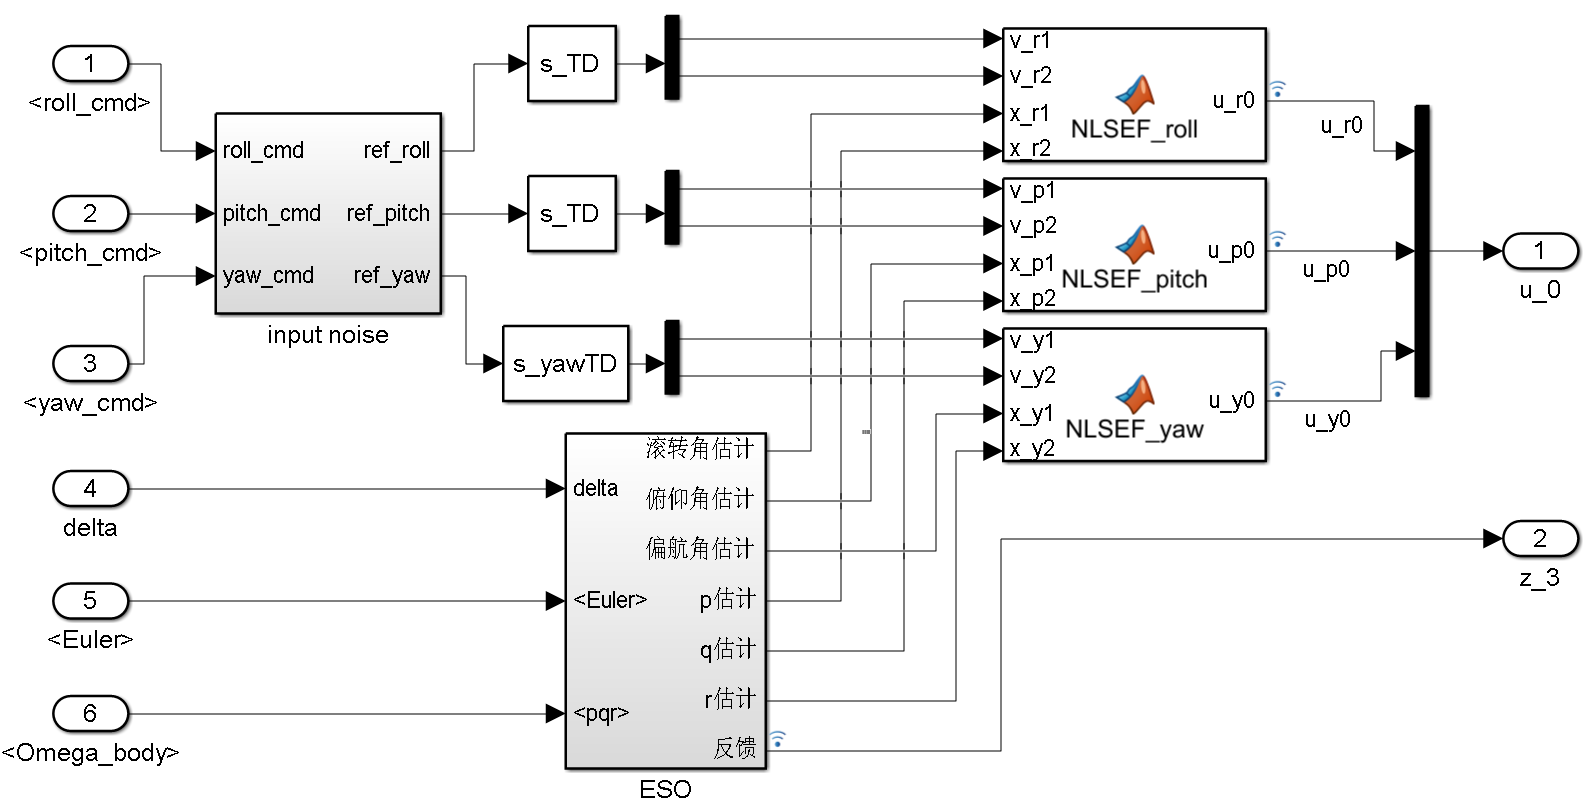
\includegraphics[scale=0.36]{Fig/Fig_Controller.png}
	\caption{\label{fig_controller_simulink}ADRC控制器仿真}
\end{figure}
\section{本章小结}
虽然在很多系统中PID控制就可以得到很满意的效果,但如本章第一节所述,在很多场合PID控制仍有诸多不足。结合所研究对象的特性,考虑使用ADRC对涵道无人机进行姿态控制。第二节介绍了ADRC的主要思想,紧接着第三节讨论了其收敛性条件并不加证明地给出几条定理。最后,第四节针对涵道无人机的姿态系统设计了ADRC控制器,应用第三节给出的定理证明了所设计的自抗扰控制收敛,并借助MATLAB$^\circledR$/Simulink$^\circledR$搭建控制器仿真。








